\section{稀疏图的构造}
\label{sec:graph-resistance-sampling}

明确了谱近似的目标后，接下来的核心问题是：\emph{如何从原图$\mathcal G$的$m$条边中只选出少量的边，构造出满足$(1-\varepsilon)\bm L_G\preceq\bm L_H\preceq(1+\varepsilon)\bm L_G$的稀疏图$\mathcal H$？}Spielman与Srivastava于2011年给出了一种随机抽样构造法：以每条边的电导与有效电阻之积$c_e R_e$作为重要性权重，从原图边集中独立有放回地抽取$q$次边，并对抽中的边按概率倒数补偿权重\scite{spielman2011graph}。本节分三步介绍抽样分布的选择、具体算法实现以及基于矩阵Chernoff界的理论证明。

\subsection{抽样分布的选择}
\label{sec:graph-resistance-sampling-distribution}

要通过随机抽边构造稀疏图，首先需要决定每条边$e\in E$在单次抽取中被选中的概率$p_e$。最朴素的想法是所有边等概率抽取（$p_e=1/m$），但它可能以很高概率漏掉维持连通性的桥边。

\paragraph{均匀抽样的风险}

考察图~\ref{fig:graph-sparsification-bridge}所示的杠铃图：左右两个稠密大团之间只有一条唯一的桥边$e_{\mathrm{bridge}}$。若在全部$m$条边中等概率独立抽样$q$次（$q\ll m$），则单次未抽中桥边的概率为$1-1/m$，连续$q$次都漏掉桥边的概率高达$(1-1/m)^q\approx\mathrm e^{-q/m}\approx 1$。

漏掉桥边会使谱近似下界不成立。为说明这一点，取一个在左团所有顶点上赋$1$、在右团所有顶点上赋$0$的测试向量$\bm x$。在左右两个团内部，每条边两端取值相同，能量贡献全为$0$；整张图在$\bm x$方向上的非零能量$\bm x^\top\bm L_G\bm x=c_{e_{\mathrm{bridge}}}>0$完全由这条桥边独自承担。漏掉桥边会使替代图在该方向上的能量变为$\bm x^\top\bm L_H\bm x=0$，直接违背谱近似要求的正下界$(1-\varepsilon)\bm x^\top\bm L_G\bm x$。

\begin{figure}[!htb]
  \centering
  \begingroup
\definecolor{SparseBridgeBlue}{HTML}{7188A3}
\definecolor{SparseBridgeBlueFill}{HTML}{E5EAF0}
\definecolor{SparseBridgeYellow}{HTML}{B4A16F}
\definecolor{SparseBridgeNeutral}{HTML}{4C4D4F}
\definecolor{SparseBridgeText}{HTML}{3B4252}
\begin{tikzpicture}[x=10mm,y=10mm,
  vertex/.style={circle,draw=SparseBridgeBlue,fill=SparseBridgeBlueFill,
    minimum size=3.2mm,inner sep=0pt,line width=.65pt},
  inneredge/.style={draw=SparseBridgeNeutral,line width=.75pt},
  bridge/.style={draw=SparseBridgeYellow,line width=1.4pt},
  text=SparseBridgeText]
  \coordinate (l1) at (0,0);
  \coordinate (l2) at (.75,.65);
  \coordinate (l3) at (1.5,0);
  \coordinate (l4) at (.75,-.65);
  \coordinate (r1) at (3.5,0);
  \coordinate (r2) at (4.25,.65);
  \coordinate (r3) at (5,0);
  \coordinate (r4) at (4.25,-.65);
  \draw[inneredge] (l1) -- (l2) -- (l3) -- (l4) -- cycle
                    (l1) -- (l3) (l2) -- (l4);
  \draw[inneredge] (r1) -- (r2) -- (r3) -- (r4) -- cycle
                    (r1) -- (r3) (r2) -- (r4);
  \draw[bridge] (l3) -- node[above,font=\footnotesize\sffamily]{桥} (r1);
  \foreach \point in {l1,l2,l3,l4,r1,r2,r3,r4}{
    \node[vertex] at (\point) {};
  }
  \node[below,font=\footnotesize] at (.75,-.87) {$x_v=1$};
  \node[below,font=\footnotesize] at (4.25,-.87) {$x_v=0$};
\end{tikzpicture}
\endgroup

  \caption{两个稠密团之间仅靠一条桥边相连。取在左团恒为$1$、右团恒为$0$的顶点函数时，两团内部边毫无能量贡献，桥边独自承担该方向的全部能量；若抽样漏掉桥边，谱近似立刻失效。}
  \label{fig:graph-sparsification-bridge}
\end{figure}

\paragraph{按有效电阻分配抽样概率}

怎样自动识别出像桥边这样决定某些方向上全部能量的边？第~\ref{sec:graph-sparsification-resistance-trees}小节建立的有效电阻与生成树理论已经给出了答案。一方面，由定理~\ref{thm:graph-tree-edge-probability}，每条边$e$的电导与有效电阻之积$c_e R_e\in(0,1]$恰好等于该边出现在随机生成树中的概率$\mathbb P(e\in T)=c_e R_e$：对于唯一的桥边，$c_e R_e=1$；而对于存在大量并联替代路径的稠密团内边，$c_e R_e$很小（如$K_n$中仅为$2/n$）。另一方面，由Foster定理（定理~\ref{thm:graph-foster-theorem}），在含$n$个顶点的连通图上，全体边的$c_e R_e$之和恒等于常数$\sum_{e\in E}c_e R_e=n-1$。

因此，将每条边的$c_e R_e$除以归一化常数$n-1$，就得到了一个合法的边抽样概率分布：
\begin{equation}
p_e=\frac{c_eR_e}{\sum_{f\in E}c_fR_f}=\frac{c_eR_e}{n-1}\qquad(e\in E).
\label{eq:graph-resistance-sampling-probability}
\end{equation}
在连通正权图（$n\geq 2$）上，每条正权边的有效电阻$R_e>0$，故$p_e>0$且$\sum_{e\in E}p_e=1$。

\paragraph{重加权补偿与单次波动界}

有了抽样概率$\{p_e\}_{e\in E}$，我们从边集中按分布$p_e$独立有放回地抽取$q$次，记第$j$次抽中的边为$e_j$（$j=1,\ldots,q$）。对于任意一条固定边$e\in E$，它在单次抽取中被选中的概率是$p_e$，$q$次抽取中平均被选中$qp_e$次。为了让它在替代图$\mathcal H$中的\emph{期望总权重}恰好等于原图权重$c_e$，规定每当边$e$被抽中一次，就给它的新权重累加$\frac{c_e}{qp_e}$（抽中概率$p_e$越小的边，一旦抽中获得的单次权重补偿越大）。将全部$q$次抽取的秩一拉普拉斯项相加，得到稀疏图$\mathcal H$的拉普拉斯矩阵：
\begin{equation}
\bm L_H
=\sum_{j=1}^q \frac{c_{e_j}}{qp_{e_j}}
     \bm b_{e_j}\bm b_{e_j}^\top.
\label{eq:graph-resistance-sampling-laplacian}
\end{equation}
沿用式~\eqref{eq:graph-sparsification-normalized-order}在正交补空间$\bm 1^\perp$上的原图能量坐标$\bm y=\bm L_G^{1/2}\bm x$，将第$j$次抽中边$e_j$所贡献的标准化秩一随机矩阵记为
\begin{equation}
\bm X_j=\frac{c_{e_j}}{qp_{e_j}}
     (\bm L_G^{-1/2}\bm b_{e_j})
     (\bm L_G^{-1/2}\bm b_{e_j})^\top.
\label{eq:graph-resistance-sampling-standardized}
\end{equation}
下面的引理揭示了有效电阻抽样分布$p_e=\frac{c_e R_e}{n-1}$如下代数性质：它不仅保证了期望无偏（$\mathbb E[\bm L_H]=\bm L_G$），而且把每一条边在最坏能量方向上的单次算子范数$\lVert\bm X_j\rVert_2$完全拉平为同一个常数$\frac{n-1}{q}$。

\begin{lemma}[有效电阻抽样的无偏性与单次范数界]
\label{lem:graph-resistance-sampling-moments}
设连通正权图按概率$p_e=c_eR_e/(n-1)$独立有放回抽取$q$次边构造式~\eqref{eq:graph-resistance-sampling-laplacian}的$\bm L_H$。则：
\begin{enumerate}
  \item 抽样矩阵的期望等于原图拉普拉斯矩阵：
  \begin{equation}
  \mathbb E[\bm L_H]=\bm L_G,\qquad
  \mathbb E\!\left[\sum_{j=1}^q\bm X_j\right]=\bm I_{\bm 1^\perp}.
  \label{eq:graph-resistance-sampling-expectation}
  \end{equation}
  \item 不论第$j$次抽中哪一条边$e_j\in E$，标准化单次矩阵$\bm X_j$都是对称半正定的，且其算子谱范数恒等于
  \[
    \lVert\bm X_j\rVert_2=\frac{n-1}{q}.
  \]
\end{enumerate}
\end{lemma}

\begin{proof}
（1）对固定的第$j$次抽样，随机矩阵$\bm Y_j=\frac{c_{e_j}}{qp_{e_j}}\bm b_{e_j}\bm b_{e_j}^\top$以概率$p_e$取值为$\frac{c_e}{qp_e}\bm b_e\bm b_e^\top$（$e\in E$）。因此单次期望为
\[
  \mathbb E[\bm Y_j]
  =\sum_{e\in E}p_e\cdot\frac{c_e}{qp_e}\bm b_e\bm b_e^\top
  =\frac{1}{q}\sum_{e\in E}c_e\bm b_e\bm b_e^\top
  =\frac{1}{q}\bm L_G.
\]
对$j=1,\ldots,q$求和即得$\mathbb E[\bm L_H]=\bm L_G$；两侧在$\bm 1^\perp$上夹乘$\bm L_G^{-1/2}$即得$\mathbb E\bigl[\sum_{j=1}^q\bm X_j\bigr]=\bm L_G^{-1/2}\bm L_G\bm L_G^{-1/2}=\bm I_{\bm 1^\perp}$。

（2）记向量$\bm v_j=\bm L_G^{-1/2}\bm b_{e_j}\in\bm 1^\perp$，则$\bm X_j=\frac{c_{e_j}}{qp_{e_j}}\bm v_j\bm v_j^\top$是正标量与向量外积的乘积，故对称半正定且秩为$1$，其唯一非零特征值（即算子范数$\lVert\bm X_j\rVert_2$）等于系数乘以$\lVert\bm v_j\rVert_2^2$。注意到$\bm v_j$的欧氏长度平方恰好就是边$e_j$两端的有效电阻：
\[
\lVert\bm v_j\rVert_2^2
=\bm b_{e_j}^\top\bm L_G^\dagger\bm b_{e_j}
=R_{e_j}.
\]
将$p_{e_j}=c_{e_j}R_{e_j}/(n-1)$代入$\lVert\bm X_j\rVert_2=\frac{c_{e_j}}{qp_{e_j}}\lVert\bm v_j\rVert_2^2$，分子与分母中的$c_{e_j}R_{e_j}$精确对消：
\[
\lVert\bm X_j\rVert_2
=\frac{c_{e_j}R_{e_j}}{qp_{e_j}}
=\frac{n-1}{q}.\qedhere
\]
\end{proof}

\subsection{算法实现}
\label{sec:graph-resistance-sampling-algorithm}

将上述抽样与重加权规则整理为如下算法。

\begin{algorithm}[按有效电阻抽样构造稀疏图]
\label{alg:graph-resistance-sampling}
输入：连通正权图$\mathcal G=(V,E,c)$的边表与各边有效电阻$\widehat R_e$（精确值或严格为正且带相对误差保证的估计值），抽样次数$q$。输出：顶点集为$V$的稀疏重加权子图$\mathcal H=(V,E_H,\widehat c)$。
\begin{enumerate}
  \item \textbf{计算抽样分布}：对每条边$e\in E$计算权重积$c_e\widehat R_e$，归一化为概率分布$p_e=c_e\widehat R_e/\sum_{f\in E}c_f\widehat R_f$，建立累计概率表并将所有边的输出权重$\widehat c_e$初始化为$0$。
  \item \textbf{独立有放回抽样与重加权}：独立重复$q$次：在$[0,1)$上生成均匀随机数，按累计概率表定位抽中的边$e$，将其输出权重累加$\widehat c_e\leftarrow\widehat c_e+c_e/(qp_e)$。
  \item \textbf{输出稀疏图}：保留全部原图顶点$V$，输出所有满足$\widehat c_e>0$的边及其累计权重$\widehat c_e$。
\end{enumerate}
\end{algorithm}

在第一步与第二步的实现中，可将区间$[0,1)$按边表顺序切分为$m$个长度分别为$p_{e_1},\ldots,p_{e_m}$的相邻子区间；每次抽取时用二分查找在$O(\log m)$时间内定位随机数落入的子区间（或用Walker别名表在$O(m)$预处理后实现每次$O(1)$时间抽样）。若算出的所需抽样次数$q\geq m$，则直接返回原图$\mathcal G$即可。

\begin{example}[四点五边图上的有效电阻抽样与重加权过程]
\label{ex:graph-resistance-sampling}
在例~\ref{ex:graph-sparsification-trees}的四点五边单位权图上演示算法~\ref{alg:graph-resistance-sampling}。四条环边的$c_e R_e=5/8$，对角边$13$的$c_e R_e=1/2$，Foster总和为$n-1=3$。归一化后得到四条环边的抽样概率均为$p_e=\frac{5/8}{3}=\frac{5}{24}$，对角边$13$的抽样概率为$p_{13}=\frac{1/2}{3}=\frac{1}{6}$。

为展示重加权规则，这里不使用$q\geq m$时返回原图的快捷处理，取演示样本数$q=6$；这一小样本演示本身不声称满足给定谱精度。每当抽中一条环边，其权重累加$\frac{1}{6\times(5/24)}=\frac{4}{5}$；每当抽中对角边$13$，其权重累加$\frac{1}{6\times(1/6)}=1$（对角边抽中概率较小，单次补偿权重更高）。

假设$6$次随机数依次抽中边$12,23,34,41,13,12$（图~\ref{fig:sparsification-sampling-intervals}标出了第$1$次和第$6$次随机数均落入边$12$的概率区间），表~\ref{tab:graph-resistance-sampling}记录了各步权重的累加过程。最终边$12$因被抽中两次而获得权重$\frac85$，其余三条环边权重为$\frac45$，对角边权重为$1$。
\end{example}

\begin{BookInlineFigure}
  \centering
  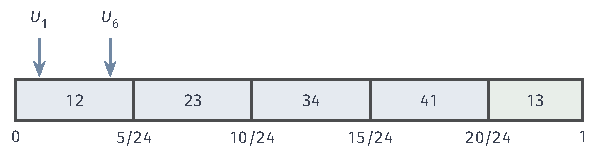
\includegraphics{figures/03-graphs/05-matrices-and-spectra/tikz/sparsification-sampling-intervals/figure.pdf}
  \caption{按各边抽样概率$p_e$切分单位区间$[0,1)$。区间内的两位数字表示边的端点。第$1$次和第$6$次的均匀随机数都落入边$12$的区间$[0,5/24)$内，因此两次增量$\frac45$均累加在边$12$上。}
  \label{fig:sparsification-sampling-intervals}
\end{BookInlineFigure}

\begin{table}[!htb]
  \centering
  \caption{四点五边图在$q=6$次抽样下的边权累加过程。}
  \label{tab:graph-resistance-sampling}
  \begin{tabular}{ccrrrrr}
    \toprule
    抽样序号 & 抽中的边 & $\widehat c_{12}$ & $\widehat c_{23}$ & $\widehat c_{34}$ & $\widehat c_{41}$ & $\widehat c_{13}$ \\
    \midrule
    1 & $12$ & $4/5$ & 0 & 0 & 0 & 0 \\
    2 & $23$ & $4/5$ & $4/5$ & 0 & 0 & 0 \\
    3 & $34$ & $4/5$ & $4/5$ & $4/5$ & 0 & 0 \\
    4 & $41$ & $4/5$ & $4/5$ & $4/5$ & $4/5$ & 0 \\
    5 & $13$ & $4/5$ & $4/5$ & $4/5$ & $4/5$ & 1 \\
    6 & $12$ & $8/5$ & $4/5$ & $4/5$ & $4/5$ & 1 \\
    \bottomrule
  \end{tabular}
\end{table}

\subsection{算法分析}
\label{sec:graph-resistance-sampling-analysis}

引理~\ref{lem:graph-resistance-sampling-moments}(1)保证了抽样图在平均意义下满足$\mathbb E[\bm L_H]=\bm L_G$；但实际算法只生成一张随机图$\mathcal H$，我们需要保证这张图以高概率\emph{同时在所有向量方向$\bm x\in\mathbb R^n$上}满足$(1-\varepsilon)\bm x^\top\bm L_G\bm x\leq\bm x^\top\bm L_H\bm x\leq(1+\varepsilon)\bm x^\top\bm L_G\bm x$。

在正交补空间$\bm 1^\perp$的能量坐标下，所有方向上的二次型能量比值都被夹在随机矩阵和$\sum_{j=1}^q\bm X_j$的最小特征值与最大特征值之间。因此，全部方向同时满足$1\pm\varepsilon$谱近似，当且仅当算子范数偏差满足$\bigl\lVert\sum_{j=1}^q\bm X_j-\bm I_{\bm 1^\perp}\bigr\rVert_2\leq\varepsilon$。下面的\term{矩阵Chernoff界}（matrix Chernoff bound）\scite{tropp2012userfriendly}专门用于控制独立随机半正定矩阵和的极端特征值偏离。

\begin{theorem}[矩阵Chernoff界的单位均值形式]
\label{thm:graph-matrix-chernoff}
设$\bm X_1,\ldots,\bm X_q$是相互独立的$d\times d$随机对称半正定矩阵，满足对每个$j$恒有$\lVert\bm X_j\rVert_2\leq r$，且期望之和为单位矩阵$\sum_{j=1}^q\mathbb E[\bm X_j]=\bm I_d$。则对任意$0<\varepsilon<1$，有
\begin{equation}
\mathbb P\!\left(
  \left\lVert\sum_{j=1}^q\bm X_j-\bm I_d\right\rVert_2>\varepsilon
\right)
\leq 2d\exp\!\left(-\frac{\varepsilon^2}{3r}\right).
\label{eq:graph-matrix-chernoff}
\end{equation}
\end{theorem}

将引理~\ref{lem:graph-resistance-sampling-moments}建立的无偏性与单次范数界$r=(n-1)/q$代入定理~\ref{thm:graph-matrix-chernoff}，立即可导出有效电阻抽样的谱稀疏化主定理。

\begin{theorem}[有效电阻抽样的谱稀疏化保证]
\label{thm:graph-resistance-sparsification}
设$\mathcal G$是含$n\geq 2$个顶点的连通正权图，给定相对误差$0<\varepsilon<1$与失败概率上限$0<\delta<1$。若按有效电阻概率$p_e=c_eR_e/(n-1)$执行算法~\ref{alg:graph-resistance-sampling}，且抽样次数$q$满足
\begin{equation}
q\geq\frac{3(n-1)}{\varepsilon^2}
         \log\frac{2(n-1)}{\delta},
\label{eq:graph-resistance-sampling-count}
\end{equation}
则输出的包含至多$\min\{m,q\}$条边的重加权子图$\mathcal H$以至少$1-\delta$的概率是$\mathcal G$的$\varepsilon$谱近似：
\[
  (1-\varepsilon)\bm L_G\preceq\bm L_H\preceq(1+\varepsilon)\bm L_G.
\]
\end{theorem}

\begin{proof}
在维数$d=n-1$的子空间$\bm 1^\perp$上考察独立随机半正定矩阵$\bm X_1,\ldots,\bm X_q$。由引理~\ref{lem:graph-resistance-sampling-moments}，有$\sum_{j=1}^q\mathbb E[\bm X_j]=\bm I_{\bm 1^\perp}$且$\lVert\bm X_j\rVert_2=(n-1)/q=r$。代入式~\eqref{eq:graph-matrix-chernoff}得
\[
\mathbb P\!\left(
  \left\lVert\sum_{j=1}^q\bm X_j-\bm I_{\bm 1^\perp}\right\rVert_2>\varepsilon
\right)
\leq 2(n-1)\exp\!\left(-\frac{q\varepsilon^2}{3(n-1)}\right).
\]
当$q$满足式~\eqref{eq:graph-resistance-sampling-count}时，右端失败概率不超过$\delta$。在概率至少为$1-\delta$的成功事件上，对任意$\bm y=\bm L_G^{1/2}\bm x\in\bm 1^\perp$都有$(1-\varepsilon)\lVert\bm y\rVert_2^2\leq\bm y^\top\bigl(\sum_{j=1}^q\bm X_j\bigr)\bm y\leq(1+\varepsilon)\lVert\bm y\rVert_2^2$，换回原坐标即得$(1-\varepsilon)\bm x^\top\bm L_G\bm x\leq\bm x^\top\bm L_H\bm x\leq(1+\varepsilon)\bm x^\top\bm L_G\bm x$。又因常向量$\bm 1$在$\bm L_G$与$\bm L_H$下的二次型均为$0$，该不等式对全体$\bm x\in\mathbb R^n$成立。
\end{proof}

若算法~\ref{alg:graph-resistance-sampling}使用的是第~\ref{sec:electrical-approximate-resistance}小节求得的近似有效电阻$\widehat R_e\in[(1-\eta)R_e,(1+\eta)R_e]$（$0\leq\eta<1$），则实际抽样概率满足$\widehat p_e\geq\frac{1-\eta}{1+\eta}p_e$，单次范数上界至多放大为$r=\frac{1+\eta}{1-\eta}\cdot\frac{n-1}{q}$。因此，将式~\eqref{eq:graph-resistance-sampling-count}中的抽样次数乘以$(1+\eta)/(1-\eta)$即可控制条件于电阻估计成功事件的抽样失败概率。当$\eta$固定且远离$1$时，这才是常数因子；若估计本身以概率至多$\delta_R$失败，则总失败概率至多为$\delta_R+\delta$。

边数为$O(n\log(n/\delta)/\varepsilon^2)$并不单独证明构造时间近线性：总成本还包含有效电阻估计、概率表预处理和抽样。采用相应的快速拉普拉斯求解器并控制求解误差，才能得到近线性的构造时间保证。
